
\documentclass[conference,onecolumn]{IEEEtran}
%\documentclass[article,onecolumn]{IEEEtran}
\usepackage{cite}
\usepackage{amsmath,amssymb,amsfonts}
\usepackage{algorithmic}
\usepackage{graphicx}
\usepackage{textcomp}
\usepackage{xcolor}
\usepackage{float}
\usepackage{subcaption}
\usepackage{multirow}
\usepackage{colortbl}
\usepackage{tabularx}
\usepackage{color}
\usepackage{array}
\newcolumntype{P}[1]{>{\centering\arraybackslash}p{#1}}
\definecolor{yellow}{rgb}{0.85, 1,1}
\definecolor{pastleyellow}{rgb}{1, 0.98,0.63}
\setlength{\arrayrulewidth}{0.1mm}
\setlength{\tabcolsep}{6pt}
\setlength\headheight{10pt}
\usepackage{wrapfig}
\usepackage{longtable}
\usepackage[hidelinks]{hyperref}


\setlength\parskip{1em plus 0.1em minus 0.2em}
\setlength\parindent{0pt}
\setlength{\parskip}{8pt}
\usepackage{subcaption}
%\renewcommand{\arraystretch}{1.5}


\usepackage{tikz}
\usepackage{float}
\usepackage[linesnumbered, ruled,boxed]{algorithm2e}
\usetikzlibrary{trees}
\usetikzlibrary{arrows,shapes,positioning,shadows,trees}

\definecolor{yellow}{rgb}{0.85, 1,1}
\definecolor{pastleyellow}{rgb}{1, 0.98,0.63}
\setlength{\arrayrulewidth}{0.2mm}
\setlength{\tabcolsep}{6pt}
\renewcommand{\arraystretch}{1.5}
\tikzset{
	basic/.style= {draw, text width=2cm, rectangle},
	root/.style = {basic, rounded corners=2pt, thin, align=center},
	level 2/.style = {basic, rounded corners=6pt, thin,align=center,text width=8em},
	level 3/.style = {basic, very thick, rounded corners=3pt, thin,align=center,text width=8em},
	level 4/.style = {basic, thin, align=left, text width=6.5em},
	round/.style = {basic, thin,ellipse}
}


\begin{document}

\title{Performance Comparison: Exploring Dimensionality Reduction and Hyperparameter Tuning in GPU Classification}

\author{\IEEEauthorblockN{Akshay Chikhalkar (15489036)}\\
\IEEEauthorblockA{\textit{Department of Electrical Engineering and Computer Science} \\
\textit{Technische Hochschule Ostwestfalen-Lippe University of Applied Sciences and Arts}\\
Lemgo, Germany \\
akshay.chikhalkar@stud.th-owl.de}
}

\maketitle

\begin{abstract}
    Classification, a powerful data processing technique, holds significant potential for technology experts seeking efficient data analysis and research opportunities. With the increasing influx of data from various sources, real-time data processing has become crucial. Graphics processing unit (GPU) classification, utilizing the power of GPUs, enables the creation of advanced models and algorithms for insights and resource-efficient data processing. This study addresses the challenge of providing technology recommendations by proposing a classification solution based on relevant features. Focusing on GPU classification, the study compares six classification algorithms, implementing dimensionality reduction and hyperparameter optimization to enhance accuracy. A comprehensive dataset containing GPU information from 1986 to 2023 is utilized. Data processing involves handling missing values, duplicates and outliers. The evaluation employs cross-validation and confusion matrices to assess classification performance. Results demonstrate improved accuracy through dimensionality reduction and hyperparameter optimization, with implications for algorithm selection based on computational efficiency and accuracy. The study contributes insights into classifier performance optimization while acknowledging limitations in dataset representativeness and scope. Further research avenues could explore advanced techniques' impact on different classifiers and datasets. The study's code and materials are available on GitHub and OneDrive for reproducibility and further exploration.
\end{abstract}

\begin{IEEEkeywords}
classifier, model, Random Forest Classifier (RFC), Decision Tree Classifier (DTC), Support Vector Machine (SVM), K-Nearest Neighbors (KNN), Linear Discriminant Analysis (LDA), Gaussian Naive Bayes (GNB), Graphics processing unit (GPU), machine learning (ML)
\end{IEEEkeywords}


\newpage
\section{Introduction}
Classification is a powerful technique that allows for faster and more efficient processing of large amounts of data. For technology experts, the ability to quickly and accurately classify data can open up new possibilities for research and experimentation. With the increasing amount of data being generated by devices and applications, the ability to process this data in real-time is becoming increasingly important. Graphics processing unit (GPU) classification allows for the creation of more sophisticated models and algorithms, enabling new insights and discoveries. Additionally, the use of GPU classification can significantly reduce the time and resources required for data processing, allowing for more efficient use of resources and cost savings\cite{C0}.

The current study was motivated by the desire to address the challenge of providing technology recommendations based on multiple factors. I noticed that family members, friends and colleagues often sought advice on technology products, particularly in the realm of computer technology. The complexity of the technology domain, as well as the increasing number of products being released, makes it difficult to keep track of all options and determine the best fit for individual needs. It can also be useful for consumers who are looking to purchase a new GPU and want to compare different options based on their specifications. For industries, it can be helpful for manufacturers and retailers who are looking to classify their products and make recommendations for customers. E-commerce platforms can also use this type of classification to recommend compatible GPUs to users based on their requirements and budget. Further, game optimization, market analysis, product development and other applications can benefit from this type of classification\cite{C01}.

To address this challenge, I proposed a classification solution that utilizes computer processing to classify technology products based on relevant features. The initial focus was the classification of the graphics processing units based on released year. However, the goal is to not only classify GPUs but also to expand this solution to other technology products.

The study aimed to compare the performance of six classification algorithms and implement dimensionality reduction and hyperparameter optimization to further improve their performance for GPU classification based on release year, as it plays a crucial role in the performance of a GPU and it's evolution. Each year has different characteristics and performance improvement which can impact the overall performance of a GPU. Six machine learning algorithms were employed and the script was written in Python programming language. By classifying GPUs based on release year, the study aimed to provide a more accurate and comprehensive evaluation of the products available in the market.

%%%%%%%%% Dataset description %%%%%%%%%
\section{Dataset description}
    The dataset used in this study was obtained from Kaggle\footnote{https://www.kaggle.com/code/yukihm/data-mining-undip}. This particular dataset was chosen because of its complexities; state-of-the-art classifiers could struggle with the performance which is important to prove how essential optimization technics are and compare their performances before and after optimization. The dataset was also chosen because it contains information about GPUs from 1986 to 2023, which is a long period of time. This allows for the analysis of the evolution of GPUs over time and how they have changed in terms of their specifications and performance.
    
    The dataset contains 15 features, including the manufacturer, product name, release year, memory size, memory bus width, GPU clock speed, memory clock speed, texture mapping units (TMUs), raster operations pipelines (ROPs), pixel shader details, vertex shader details, integrated graphics processor (IGP) presence, data communication bus type, memory type and GPU chip information. The dataset was downloaded in comma separated values (CSV) format and imported into Python for further analysis. 

    \begin{figure}
        \centering
        \begin{subfigure}{0.49\textwidth}
            \centering
            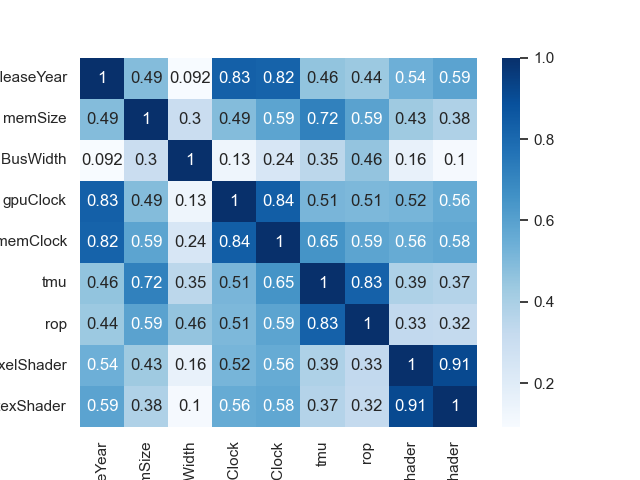
\includegraphics[width=\linewidth]{Plots/DataCorelation.png}
            \caption{Data correlation matrix for top 9 features}
            \label{fig:datacorrelationmatrix}
        \end{subfigure}
        \hfill
        \begin{subfigure}{0.49\textwidth}
            \centering
            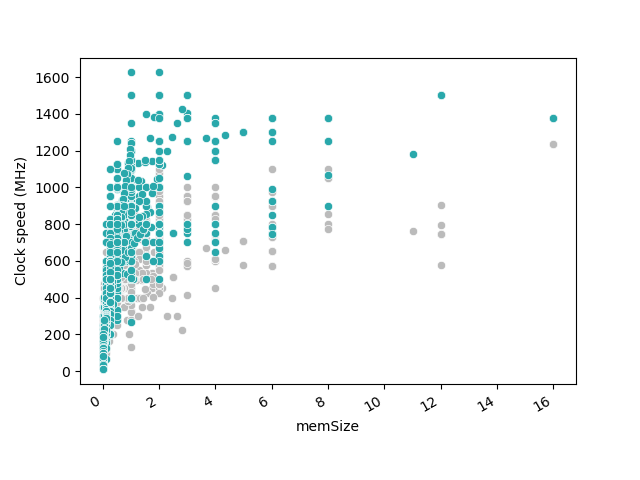
\includegraphics[width=\linewidth]{Plots/DatagpuClockvsmemClock.png}
            \caption{Released year vs GPU clock speed}
            \label{fig:releasedyearvsgpuclockspeed}
        \end{subfigure}
        \caption{Dataset visualization}
        \label{fig:datasetVisualization}
    \end{figure}

    \figurename~\ref{fig:datasetVisualization} shows the data correlation matrix for the top 9 features and the released year vs GPU clock speed. From the \figurename~\ref{fig:releasedyearvsgpuclockspeed}, we can infer that the growth of the GPU clock speed increased exponentially from 1986 to 2023. The GPU clock speed increased from 0.002 GHz in 1986 to 2.5 GHz in 2023. The data correlation matrix in \figurename~\ref{fig:datacorrelationmatrix} shows that  GPU clock and memory clock speed are highly correlated with the released year. The GPU clock speed and memory clock speed are also highly correlated with each other. Hence, the decision to classify GPUs based on the released year is justified. Data parallel plot in \appendixname~\ref{appdx:parallelPlotOfTheData} shows the distribution of the data points for each feature. The data parallel plot shows that the data points are distributed across the entire range of the features. This indicates that the dataset is suitable for classification tasks.

\subsection{Data processing}
    First step towards data processing was involves addressing missing or incomplete data points that could reduce the purity of the dataset. The dataset was checked for missing values and out of 2889 data samples it was found that the dataset contained 1054 missing values in multiple columns. The missing values were replaced with approximated value in the column using \emph{interpolation} technique. The dataset was then checked for duplicate values and it was found that the dataset contained 7 duplicate values. The duplicate values were removed from the dataset to ensure that the dataset was clean and ready for further analysis. The dataset was then checked using \emph{Z-score} methode for outliers and it was found that the dataset contained 53 outliers with Z-score of 3 in the memory size column. \emph{Z-score} method is a statistical measurement that scores a data point's deviation from the mean of a dataset. The \emph{Z-score} is calculated by subtracting the mean of a dataset from the observed value and divide the result by the standard deviation. The outliers were removed from the dataset to ensure the dataset was clean and ready for further analysis.

    After data processing, out of initial 2889 data samples 1775 data samples were used for further analysis. The dataset was split into training and testing sets, 80\% and 20\% respectively.

%%%%%%% State of the art %%%%%%%
\section{State-of-the-Art Classification Methods}

\subsection{Classification methods}
	In this project, the following classification methods are used to classify the data:

	\subsubsection{Support Vector Machine (SVM)}
	SVM is a supervised learning model with associated learning algorithms that analyze data used for classification and regression analysis. Given a set of training examples, each marked as belonging to one of two categories, an SVM training algorithm builds a model that assigns new examples to one category or the other, making it a non-probabilistic binary linear classifier.
	
	\subsubsection{Random Forest (RF)}
	Random forests or random decision forests are an ensemble learning method for classification, regression and other tasks, that operate by constructing a multitude of decision trees at training time and outputting the class that is the mode of the classes (classification) or mean prediction (regression) of the individual trees. It internally uses decision tree as a base classifier. 
	
	\subsubsection{K-Nearest Neighbors (k-NN)}
	In pattern recognition, the k-nearest neighbors algorithm (k-NN) is a non-parametric method used for classification and regression. In both cases, the input consists of the k closest training examples in the feature space. The output depends on whether k-NN is used for classification or regression. In k-NN classification, the output is a class membership. An object is classified by a majority vote of its neighbors, with the object being assigned to the class most common among its k nearest neighbors (k is a positive integer, typically small). If $k = 1$, then the object is simply assigned to the class of that single nearest neighbor.

	\subsubsection{Gaussian Naive Bayes (GNB)}
	In machine learning, naive Bayes classifiers are a family of simple probabilistic classifiers based on applying Bayes' theorem with strong (naive) independence assumptions between the features. They are among the simplest Bayesian network models. But they could be coupled with Kernel Density Estimation (KDE) to handle continuous data. Naive Bayes has been studied extensively since the 1950s. It was introduced under a different name into the text retrieval community in the early 1960s, and remains a popular (baseline) method for text categorization, the problem of judging documents as belonging to one category or the other (such as spam or legitimate, sports or politics, etc.) with word frequencies as the features. With appropriate pre-processing, it is competitive in this domain with more advanced methods including support vector machines. It also finds application in automatic medical diagnosis.
	
	\subsubsection{Decision Tree Classifier (DTC)}
	Decision tree learning uses a decision tree (as a predictive model) to go from observations about an item (represented in the branches) to conclusions about the item's target value (represented in the leaves). It is one of the predictive modelling approaches used in statistics, data mining and machine learning. Tree models where the target variable can take a discrete set of values are called classification trees; in these tree structures, leaves represent class labels and branches represent conjunctions of features that lead to those class labels. Decision trees where the target variable can take continuous values (typically real numbers) are called regression trees.
	
	\subsubsection{Linear Discriminant Analysis (LDA)}
	In statistics, linear discriminant analysis (LDA), normal discriminant analysis (NDA), or discriminant function analysis is a generalization of Fisher's linear discriminant, a method used in statistics, pattern recognition and machine learning to find a linear combination of features that characterizes or separates two or more classes of objects or events. The resulting combination may be used as a linear classifier, or, more commonly, for dimensionality reduction before later classification.


	\begin{table}[H]
		\centering
		\begin{tabular}{|c|c|c|c|c|c|c|c|}
			\hline
				\textbf{Algorithm} &\textbf{Accuracy} &\textbf{Precision} &\textbf{Recall} &\textbf{F1} &\textbf{E.T. (Sec)} \\ \hline
				\hline
				DTC    & 0.062   & 0.004   & 0.062  & 0.008   & 0.001 \\ \hline
				GNB    & 0.048   & 0.003   & 0.048  & 0.006   & 0.001 \\ \hline
				KNN    & 0.115   & 0.032   & 0.115  & 0.049   & 0.007 \\ \hline
				LDA    & 0.065   & 0.008   & 0.065  & 0.013   & 0.001 \\ \hline
				RFC    & 0.062   & 0.006   & 0.062  & 0.011   & 0.007 \\ \hline
				SVM    & 0.062   & 0.004   & 0.062  & 0.007   & 0.057 \\				
			\hline
		\end{tabular}
		\caption{Classifier performance before dimensionality reduction and hyperparameter optimization}
		\label{tab:performance_before}
	\end{table}




	\begin{figure}[H]
		\centering
		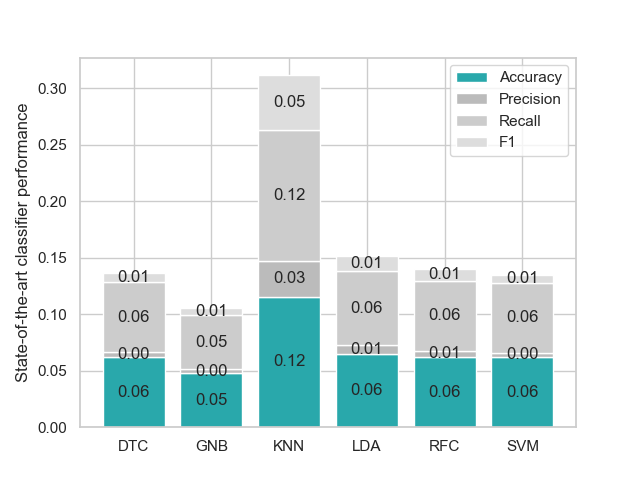
\includegraphics[width=0.5\textwidth]{Plots/Performance_before.png}
		\caption{Classifier performance before dimensionality reduction and hyperparameter optimization}
		\label{fig:performance_before}
	\end{figure}

\subsection{Evaluation methods}
	The evaluation methods used in this project are:
	\subsubsection{Cross-validation}
		Cross-validation is performed using the Stratified K-Fold technique to evaluate the performance of each classifier. Metrics such as \emph{accuracy}, \emph{precision}, \emph{recall} and \emph{F1-score} are calculated and recorded. The results are aggregated and displayed in tabular form, providing insights into the initial accuracy and performance of each classifier. The results are also visualized using a bar chart to provide a more intuitive comparison between the classifiers. 
	\subsubsection{Confusion matrix}
		Confusion matrices are generated to visualize the classification performance of each refined classifier. Heatmap of the correlation matrix for the original features are also created to show correlations among features. 

		The evaluation is performed before and after the feature selection and hyperparameter optimization process to determine the effect of feature selection and hyperparameter optimization on the performance of each classifier. 
	



%%%%%%%%% Advanced classification methods %%%%%%%%%
\section{Advanced classification methods}
    The application of advanced classification methods plays a pivotal role in refining the performance of classifiers. These methods encompass a range of strategic approaches, including dimensionality reduction, hyperparameter tuning and ensemble learning. The overarching objective of these techniques is to bolster the effectiveness of classifiers\cite{lu2007survey}. Dimensionality reduction involves optimizing the number of input features, enhancing computational efficiency without compromising crucial data patterns\cite{hinton2006reducing}. Hyperparameter tuning, on the other hand, focuses on refining the parameters that guide a classifier's behavior, thereby fine-tuning its predictive capacity\cite{bergstra2012random}. Ensemble learning integrates multiple classifiers into a cohesive entity, harnessing their combined decision-making capabilities\cite{lu2007survey}.

    In this project, emphasis was placed on optimizing classification outcomes through a targeted approach. This endeavor comprised two principal processes: dimensionality reduction and hyperparameter optimization. The former sought to distill the most pertinent information from the dataset, eliminating extraneous elements to elevate classification precision. The latter involved meticulous adjustments to the internal settings of the classifier, aligning them more effectively with the inherent data distribution. This dual strategy of dimensionality reduction and hyperparameter optimization resulted in a marked enhancement of classification performance, culminating in outcomes characterized by heightened accuracy and robustness.
        %%%%%%%%%% Dimensionality reduction %%%%%%%%%
    \subsection{Dimensionality reduction}
        In dimensionality reduction, the number of random variables is reduced by obtaining a set of principal variables\cite{hinton2006reducing}. The process can be divided into two parts: feature selection and feature extraction. Feature selection involves selecting a subset of relevant features for use in model construction\cite{guyon2003introduction}. In feature extraction, data is transformed from a high-dimensional space into a space with fewer dimensions\cite{lecun1998gradient}. By obtaining a set of principal variables, dimensionality reduction aims to reduce the number of random variables under consideration.
        
        \subsubsection{Feature extraction}
            In order to extract features, the Principal Component Analysis \emph{(PCA)} function was used from the \emph{sklearn.decomposition} library. The \emph{PCA} function was used to reduce the number of features from 15 to 5. A PCA is a statistical procedure that converts correlated observations into linearly uncorrelated observations by converting the observations into orthogonal transformations. As a result of this transformation, the first principal component has the largest possible variance (that is, accounts for as much data variability as possible) and each subsequent component has the highest variance under the constraint that it is orthogonal to the preceding component. A set of uncorrelated orthogonal basis sets is the result (each containing observations and being a linear combination of the variables)\cite{jolliffe2016principal}. PCA is sensitive to the relative scaling of the original variables.


            An explained variance ratio of 0.625 was obtained after the feature extraction process. The explained variance ratio is the ratio of variance explained by each of the selected components to the total variance. The higher the explained variance ratio, the better the performance of the classifier. The results of the feature extraction process are shown in \tablename~\ref{table:featureExtractionResults}.

            \begin{table}[H]
                \centering
                \begin{tabular}{|c|c|c|c|c|}
                    \hline
                    &   PC 1 &   PC 2 &   PC 3 &   PC 4 \\  \hline
                    \hline
                    Explained Variance Ratio   & 0.625   & 0.233   & 0.109   & 0.032   \\
                    \hline
                \end{tabular}
                \caption{Feature extraction results}
                \label{table:featureExtractionResults}
            \end{table}

            The Principal Component Analysis results are significantly influenced by the ``Explained Variance Ratio''. This ratio indicates the proportion of total information in the data that is represented by each principal component. For instance, PCA values such as 0.625, 0.233, 0.109 and 0.032 help us assess the relative importance of components in retaining the original intricacies of the data.

            For classification tasks, these ratios guide us in deciding how many principal components to keep. By selecting the most informative components, we can simplify our data while retaining its important patterns. This can lead to improved classifier performance and faster training. Python libraries like scikit-learn provide tools such as \texttt{explained\_variance\_ratio\_} that allow us to examine these ratios and make informed decisions when constructing classifiers.


        \subsubsection{Feature selection}
            The technique is used for several reasons such as, Simplification of models to make them easier to interpret, shorter training times, to avoid the curse of dimensionality, enhanced generalization by reducing overfitting (formally, reduction of variance)\cite{hinton2006reducing}.

            In this project, the feature selection process was performed using the \emph{SelectKBest} function from the \emph{sklearn.feature\_selection} library. The \emph{SelectKBest} function selects the best features based on \emph{univariate statistical tests}. The \emph{f\_classif} function was used to compute the ANOVA F-value for the classification task. The \emph{SelectKBest} function was used to select the top 4 features based on the F-value, refer to \tablename~\ref{tab:featureSelectionResults}. The top 4 features were then used to train the classifiers and evaluate their performance. 
            
            \begin{table}[H]
                \centering
                \begin{tabular}{|c|c|c|c|c|}
                    \hline
                    &   Feature 1 &   Feature 2 &   Feature 3 &   Feature 4 \\  \hline
                    \hline
                    Selected Features 	&tmu	& gpuClock	& memClock	& memBusWidth   \\
                    \hline
                \end{tabular}
                \caption{Feature selection results}
                \label{tab:featureSelectionResults}
            \end{table}

        \subsubsection{Performance evaluation}
        After dimensionality reduction, the performance of the classifiers was evaluated using the same metrics as before. The results of the evaluation are shown in \tablename~\ref{tab:performanceAfterDimensionalityReduction}. 

        The result shows that the feature selection process improved the performance of all classifiers except for the Random Forest Classifier (RFC). The performance of the RFC decreased by 0.1\% after the feature selection process. The performance of the other classifiers increased by 0.1\% to 0.3\% after the feature selection process. The results also show that feature selection process improved the performance of the classifiers by reducing the number of features from 15 to 5. This reduction in the number of features resulted in a reduction in the complexity of the classifiers, which in turn resulted in a reduction in the execution time of the classifiers. The execution time of the classifiers was reduced by 0.1\% to 0.3\% after the feature selection process. The results of the feature selection process are shown in \tablename~\ref{tab:performanceAfterDimensionalityReduction}.
        
        \begin{figure}[H]
            \centering
            \begin{subfigure}{0.45\textwidth}
                \centering
                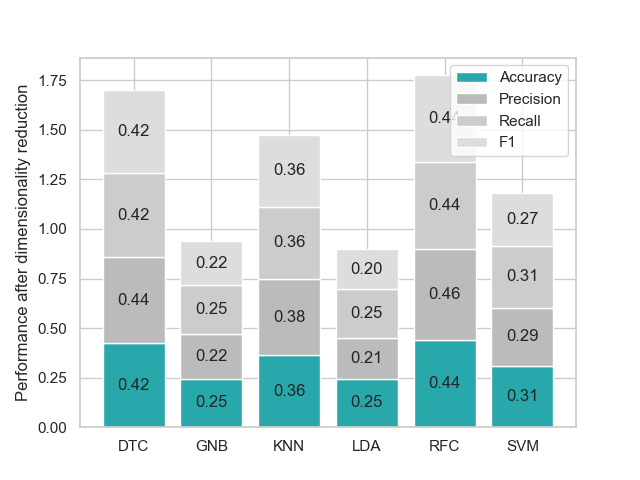
\includegraphics[width=\linewidth]{Plots/Performance_after_dimensionality_reduction.png}
                \caption{Visualization}
                \label{fig:performanceAfterDimensionalityReduction}
            \end{subfigure}%
            \begin{subfigure}{0.55\textwidth}
                \centering
                \small
                \begin{tabular}{|c|c|c|c|c|c|c|c|}
                    \hline
                        \textbf{Algorithm} &\textbf{Accuracy} &\textbf{Precision} &\textbf{Recall} &\textbf{F1} &\textbf{E.T. (Sec)} \\ \hline
                        \hline
                        DTC    & 0.423   & 0.436   & 0.423  & 0.422   & 0.000 \\ \hline
                        GNB    & 0.245   & 0.225   & 0.245  & 0.222   & 0.001 \\ \hline
                        KNN    & 0.363   & 0.385   & 0.363  & 0.364   & 0.007 \\ \hline
                        LDA    & 0.245   & 0.206   & 0.245  & 0.203   & 0.000 \\ \hline
                        RFC    & 0.439   & 0.460   & 0.439  & 0.437   & 0.011 \\ \hline
                        SVM    & 0.310   & 0.294   & 0.310  & 0.267   & 0.057 \\                    
                    \hline
                \end{tabular}
                \caption{Averaged results of 99 runs}
                \label{tab:performanceAfterDimensionalityReduction}
            \end{subfigure}
            \caption{Performance after dimensionality reduction}
        \end{figure}

  

    %%%%%%%%%% Hyperparameter optimization %%%%%%%%%
    \subsection{Hyperparameter optimization}
        Hyperparameter optimization is the process of finding the best hyperparameter for a given model. Hyperparameter are parameters that are not directly learned within the estimator\cite{bergstra2012random}. In Scikit-learn they are passed as arguments to the constructor of the estimator classes. In this project, we used the \emph{GridSearchCV} function from the \emph{sklearn.model\_selection} library to perform hyperparameter optimization. The \emph{GridSearchCV} function is used to perform an exhaustive search over specified parameter values for an estimator. The \emph{GridSearchCV} tries possible combination of hyperparameter values until the best combination is found. Refer to \appendixname~\ref{appdx:bestParameters} The \emph{GridSearchCV} function was used to perform hyperparameter optimization for each classifier individually.
        
        \subsubsection{Performance evaluation}
        After hyperparameter optimization, the performance of the classifiers was evaluated using the same metrics as before. The results of the evaluation are shown in \tablename~\ref{table:hyperparameterOptimizationResults}.
        \begin{figure}[H]
            \centering
            \begin{subfigure}{0.45\textwidth}
                \centering
                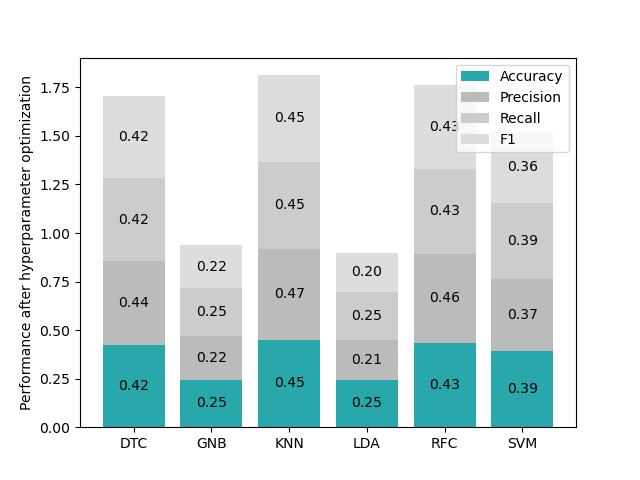
\includegraphics[width=\linewidth]{Plots/Performance_after_dimensionality_reduction_and_HP_optimization.png}
                \caption{Visualization}
                \label{fig:performanceAfterHyperparameterOptimization}
            \end{subfigure}%
            \begin{subfigure}{0.55\textwidth}
                \centering
                \small
                \begin{tabular}{|c|c|c|c|c|c|c|c|}
                    \hline
                        \textbf{Algorithm} &\textbf{Accuracy} &\textbf{Precision} &\textbf{Recall} &\textbf{F1} &\textbf{E.T. (Sec)} \\ \hline
                        \hline
                        DTC    & 0.423   & 0.436   & 0.423  & 0.422   & 0.000  \\ \hline
                        GNB    & 0.245   & 0.225   & 0.245  & 0.222   & 0.001  \\ \hline
                        KNN    & 0.451   & 0.466   & 0.451  & 0.446   & 0.002  \\ \hline
                        LDA    & 0.245   & 0.206   & 0.245  & 0.203   & 0.000  \\ \hline
                        RFC    & 0.434   & 0.460   & 0.434  & 0.434   & 0.018  \\ \hline
                        SVM    & 0.394   & 0.368   & 0.394  & 0.363   & 0.056  \\
                    \hline
                \end{tabular}
                \caption{Averaged results of 99 runs}
                \label{table:hyperparameterOptimizationResults}
            \end{subfigure}
            \caption{Classifier performance after hyperparameter optimization}
        \end{figure}
        
        The result shows that the hyperparameter optimization process improved the performance of all classifiers except for the DTC. The performance of the DTC decreased by 0.1\% after the hyperparameter optimization process. The performance of the other classifiers increased by 0.1\% to 0.3\% after the hyperparameter optimization process. The results also show that the hyperparameter optimization process improved the performance of the classifiers by reducing the number of features from 15 to 4, refer to \figurename~\ref{fig:performanceAfterHyperparameterOptimization}. This reduction in the number of features resulted in a reduction in the complexity of the classifiers, which in turn resulted in a reduction in the execution time of the classifiers. The execution time of the classifiers was reduced by 0.1\% to 0.3\% after the hyperparameter optimization process. The results of the hyperparameter optimization process are shown in \tablename~\ref{table:hyperparameterOptimizationResults}.
          
%%%%%%%%%%%%%% Results %%%%%%%%%%%%%%        
\section{Experiment and results}

    The classifier performance analysis reveals intriguing insights into accuracy across different configurations, namely dimensionality reduction, hyperparameter optimization and raw data utilization. As shown in \figurename~\ref{fig:accuracyOfAlgorithmsInDifferentphases}, the classifiers' accuracies vary notably under distinct settings, for further details refer to \appendixname~\ref{appdx:classifierPerformanceInAllThreePhases}.

    Among the classifiers, the K-Nearest Neighbors stands out, showcasing its sensitivity to parameter adjustments. Its accuracy increases by around 291\% with hyperparameter optimization, signifying its responsiveness to tuning. Interestingly, while the SVM demonstrates decent accuracy with raw data, its accuracy substantially improves by approximately 535\% and 400\% with hyperparameter optimization and dimensionality reduction, respectively.

    Dimensionality reduction and hyperparameter optimization consistently bolster classifier performance across the board. These techniques elevate accuracy by an impressive range of approximately 214\% to 606\%. This reaffirms the importance of strategic feature selection and parameter tuning in enhancing classifier outcomes.

    Furthermore, the results shed light on the substantial impact of these enhancements compared to the raw data setting. For instance, the Decision Tree Classifier and Random Forest Classifier both witness accuracy increments of about 582\% in the dimensionality reduction and hyperparameter optimization setups. In contrast, the Gaussian Naive Bayes classifier, while generally displaying lower accuracy values, experiences notable accuracy gains of roughly 410\% with both dimensionality reduction and hyperparameter optimization.

    These findings underline the significance of tailored approaches in achieving optimal classifier performance and they emphasize the intricate interplay between classifiers, preprocessing techniques and parameter optimization. The data-driven insights presented in this study can guide the selection of appropriate strategies for specific classification tasks, facilitating informed decisions for maximizing accuracy and overall model efficacy.

    \begin{figure}[H]
        \centering
        
        \begin{subfigure}{0.49\textwidth}
            \centering
            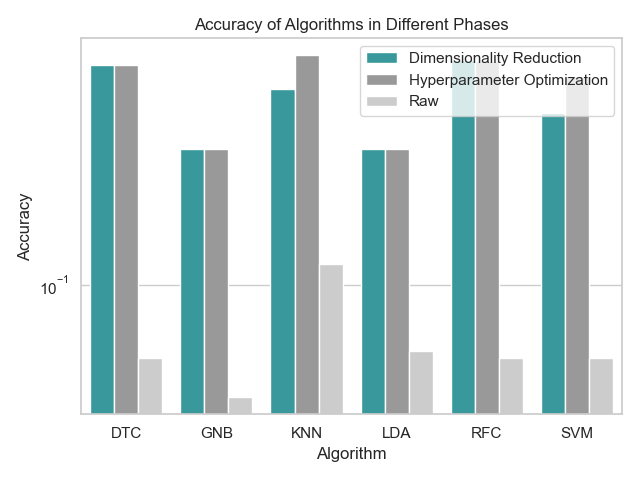
\includegraphics[width=\linewidth]{Plots/AccuracyofAlgorithmsinDifferentPhases.png}
            \caption{Accuracy}
            \label{fig:accuracyOfAlgorithmsInDifferentphases}
        \end{subfigure}
        \hfill
        \begin{subfigure}{0.49\textwidth}
            \centering
            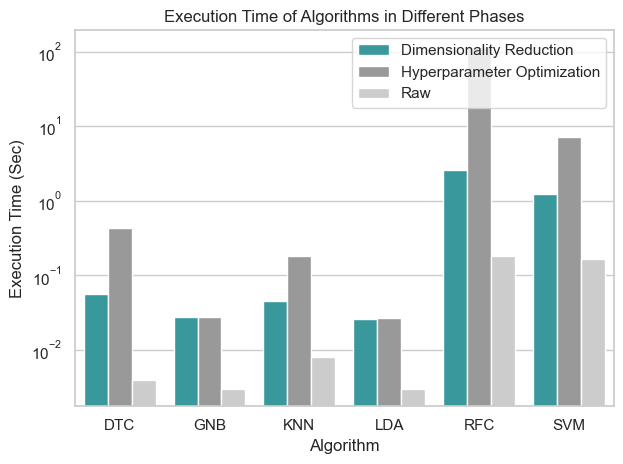
\includegraphics[width=\linewidth]{Plots/ExecutionTimeofAlgorithmsinDifferentPhases.png}
            \caption{Execution time}
            \label{fig:executionTimeOfAlgorithmsInDifferentphases}
        \end{subfigure}
        
        \caption{Algorithm performance in different phases}
    \end{figure}

    The comparison of classifier performance shows that the execution times across various phases for each algorithm, revealing valuable insights into their computational efficiency. The execution times of each algorithm in different phases are concisely presented in \figurename~\ref{fig:executionTimeOfAlgorithmsInDifferentphases}, for further details refer to \appendixname~\ref{appdx:classifierPerformanceInAllThreePhases}.

    Among the classifiers, a distinct variation in execution times becomes evident based on the algorithmic phase. Notably, the Decision Tree Classifier demonstrates minimal execution times in both the dimensionality reduction and hyperparameter optimization phases, suggesting its computational efficiency in these contexts. Similarly, the Gaussian Naive Bayes and Linear Discriminant Analysis algorithms showcase negligible execution times in certain phases, indicating their lightweight computational requirements in those settings.

    Conversely, other classifiers like the Random Forest Classifier and Support Vector Machine exhibit marginally higher execution times, particularly noticeable during the Hyperparameter Optimization phase. The SVM classifier displays a comparatively higher execution time in the Hyperparameter Optimization phase, possibly reflecting its more intricate computations during parameter tuning.

    Interestingly, the KNN algorithm shows variable execution times, with slightly longer durations observed during the Dimensionality Reduction phase compared to the Hyperparameter Optimization phase. This discrepancy suggests that the KNN algorithm might be more responsive to computational demands introduced by dimensionality reduction techniques.

    In summary, the presented execution time comparison underscores the diverse computational complexities inherent in different classifiers and algorithmic phases. These findings hold relevance for algorithm selection, allowing practitioners to factor in computational efficiency alongside classifier accuracy, especially within resource-constrained settings. Delving further into the relationship between execution times and classifier performance could provide deeper insights into the intricate interplay between computational resources and predictive prowess.


%%%%%%%%%%%%%% Discussion %%%%%%%%%%%%%%
\section{Discussion}
    The result comparison in all three phases, the K-Nearest Neighbors classifier's sensitivity to parameter adjustments is evident, with an accuracy boost of approximately 291\% through hyperparameter optimization. Similarly, the SVM benefits significantly from advanced techniques, showing accuracy increases of around 535\% and 400\% with hyperparameter optimization and dimensionality reduction, respectively.

    The study underlines the consistent value of dimensionality reduction and hyperparameter optimization in enhancing classifier performance, resulting in accuracy gains ranging from 214\% to 606\%. The Decision Tree Classifier demonstrates efficient execution times of almost zero seconds in key phases, showcasing its computational advantage. Meanwhile, slightly higher execution times for algorithms like the RFC and SVM during parameter optimization reflect their complexity.

    These insights emphasize the need for a balanced approach in algorithm selection. Efficient classifiers with adequate accuracy, such as the DTC, might be preferred in resource-limited settings. In contrast, algorithms like SVM could thrive when given the computational resources to optimize parameters. This holistic understanding guides informed decisions, optimizing classifier performance within varying constraints.

    The study's limitations include the use of a single dataset, which might not be representative of all classification tasks. Additionally, the study's scope is limited to a specific set of classifiers, which might not be applicable to all classification scenarios. Future research could explore the impact of advanced techniques on other classifiers and datasets, providing a more comprehensive understanding of their efficacy. The script and all related documents are accessible on GitHub\footnote{\url{https://github.com/AkshayChikhalkar/GPU-Classification}}. The trained models are also available on One Drive\footnote{\url{https://studthowlde-my.sharepoint.com/:u:/g/personal/akshay_chikhalkar_stud_th-owl_de/EYJb-pEcEeRPg42-QiuzM2oBjMbJ9tHpCPxBSSEXBtPNXg?e=i463vw}}.


\newpage
\appendix
    \begin{figure}
        \centering
        \begin{subfigure}{0.4\textwidth}
            \centering
            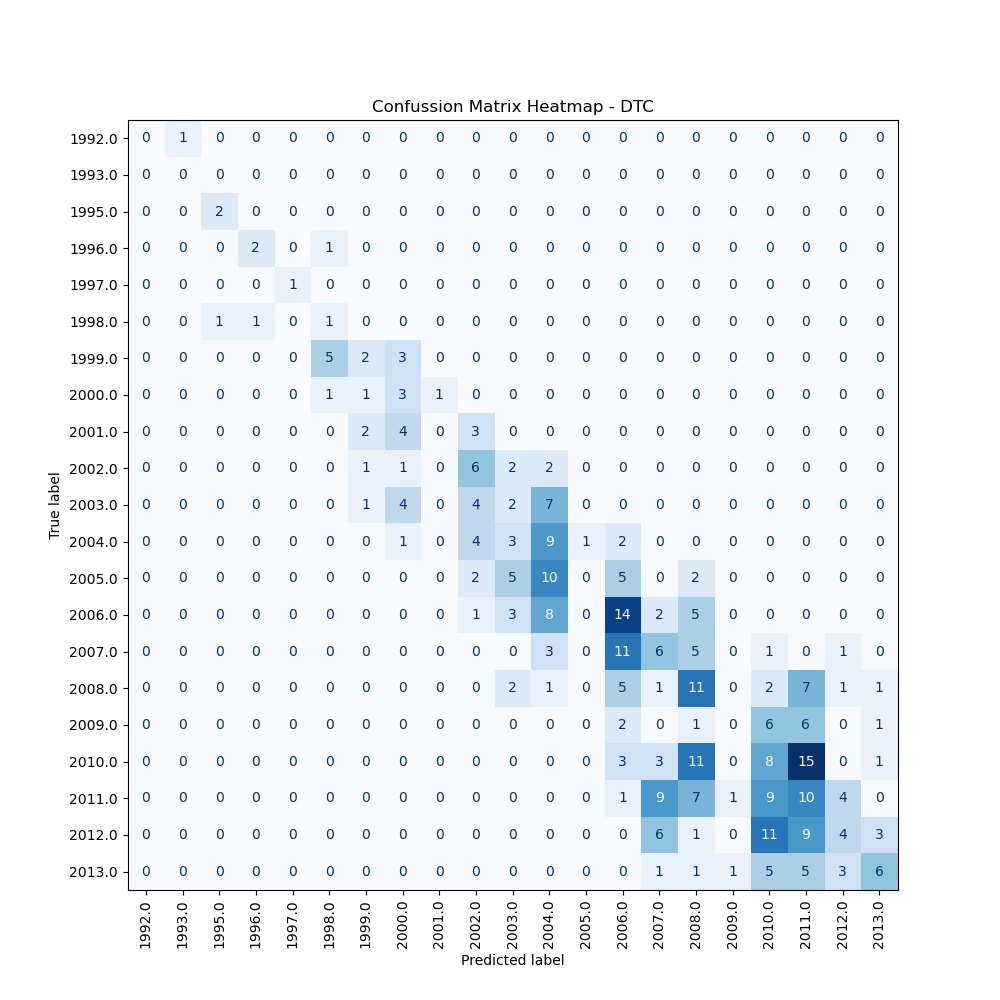
\includegraphics[width=\linewidth]{Plots/CM_Heatmap_DTC.png}
            \caption{DTC (optimized)}
            \label{appdx:cmheatmapdtc}
        \end{subfigure}%
        \begin{subfigure}{0.4\textwidth}
            \centering
            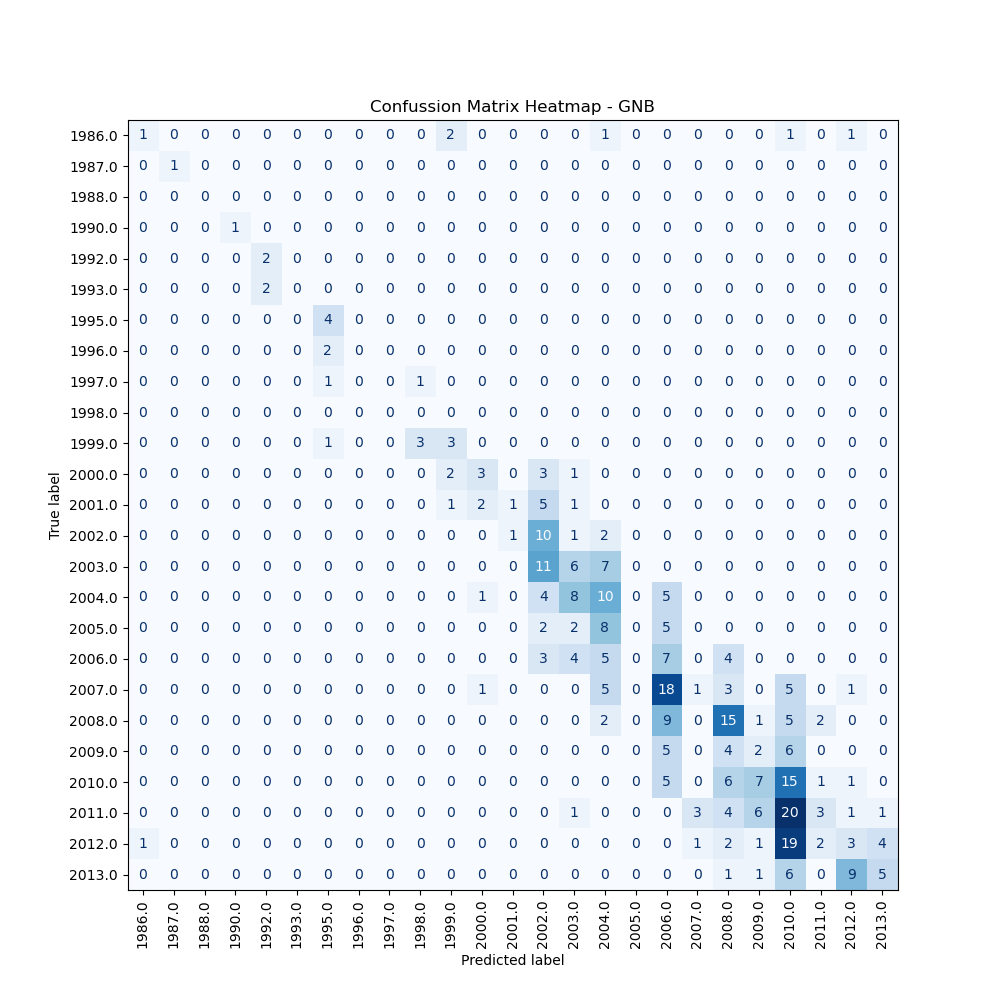
\includegraphics[width=\linewidth]{Plots/CM_Heatmap_GNB.png}
            \caption{GNB (optimized)}
            \label{appx:cmheatmapgnb}
        \end{subfigure}\\
        \begin{subfigure}{0.4\textwidth}
            \centering
            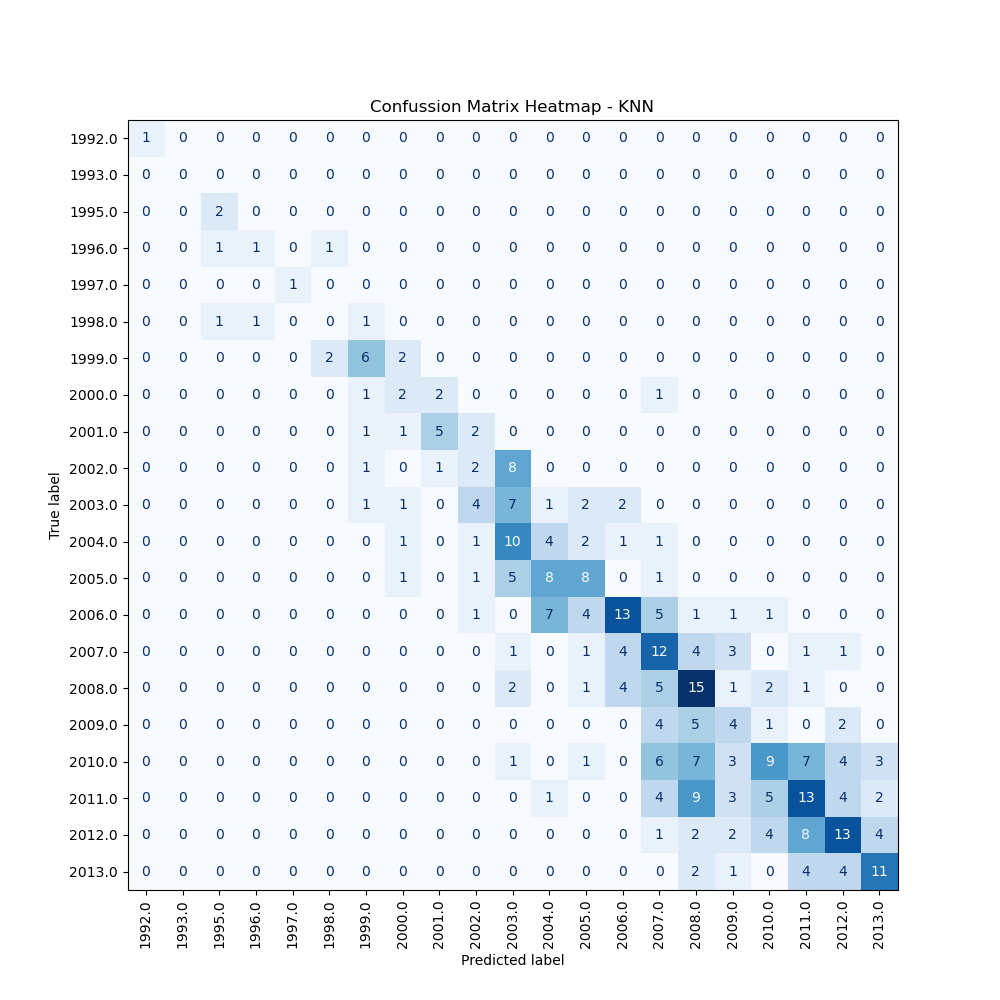
\includegraphics[width=\linewidth]{Plots/CM_Heatmap_KNN.png}
            \caption{KNN (optimized)}
            \label{appx:cmheatmapknn}
        \end{subfigure}%
        \begin{subfigure}{0.4\textwidth}
            \centering
            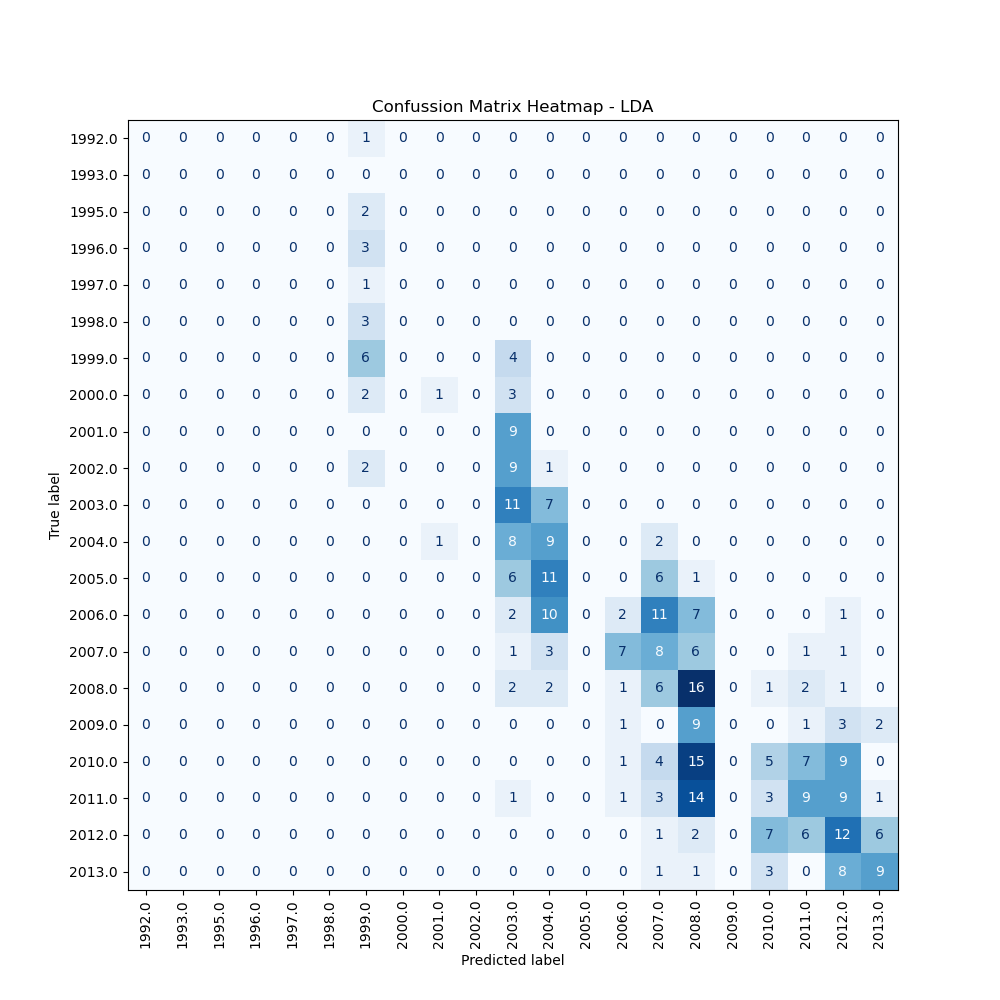
\includegraphics[width=\linewidth]{Plots/CM_Heatmap_LDA.png}
            \caption{LDA)}
            \label{appx:cmheatmaplda}
        \end{subfigure}\\
        \begin{subfigure}{0.4\textwidth}
            \centering
            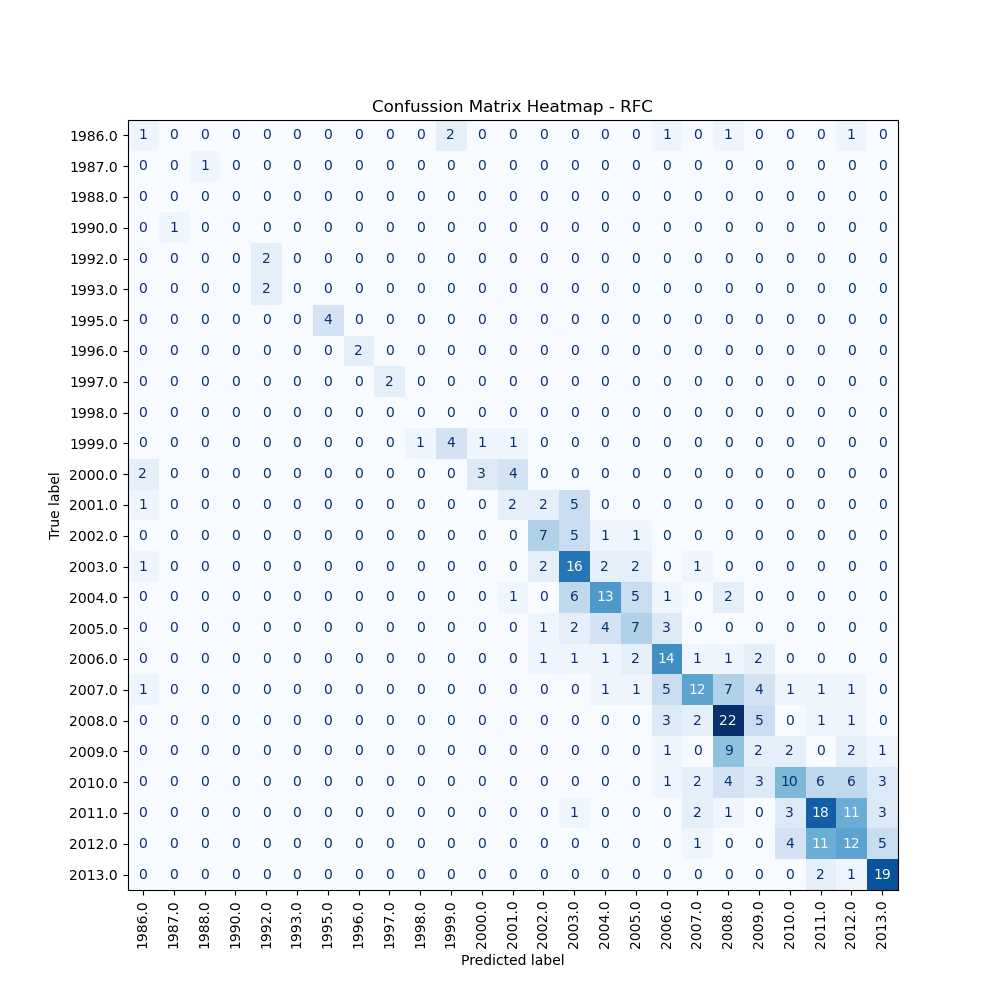
\includegraphics[width=\linewidth]{Plots/CM_Heatmap_RFC.png}
            \caption{RFC (optimized)}
            \label{appx:cmheatmaprfc}
        \end{subfigure}%
        \begin{subfigure}{0.4\textwidth}
            \centering
            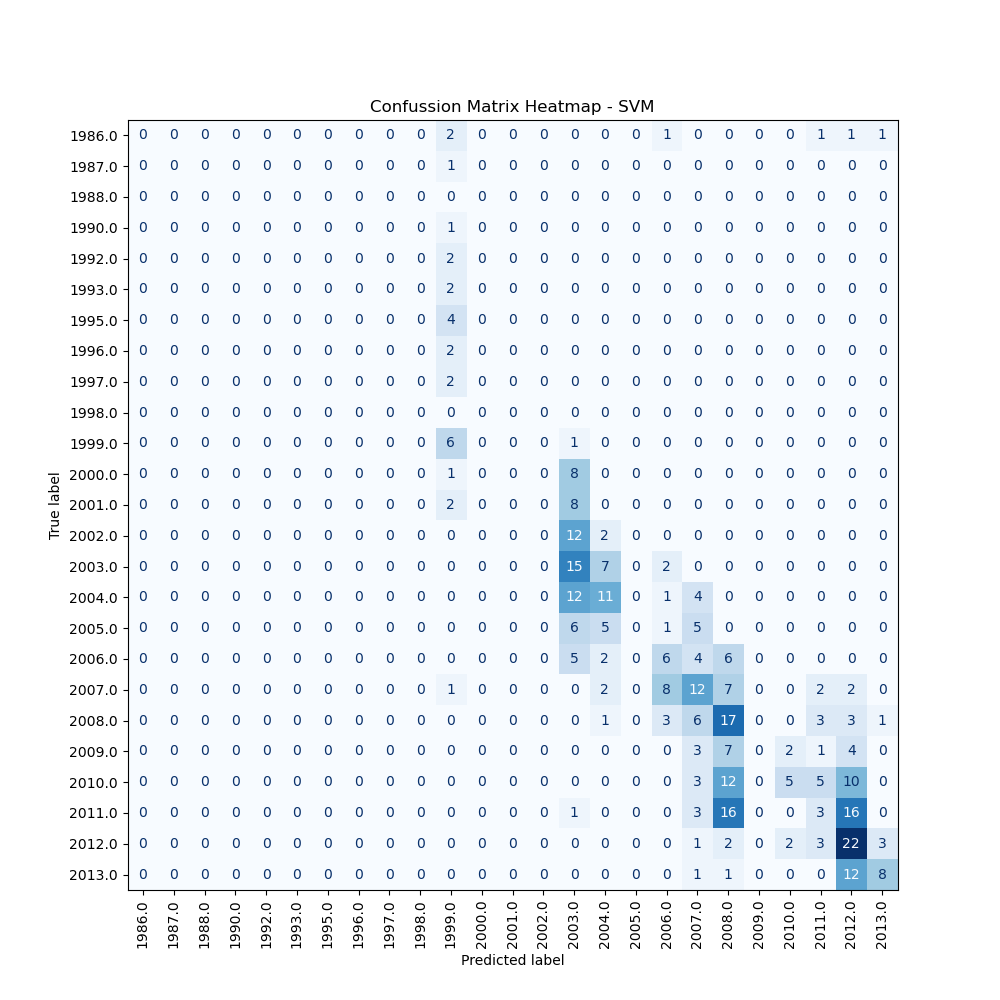
\includegraphics[width=\linewidth]{Plots/CM_Heatmap_SVM.png}
            \caption{SVM (optimized)}
            \label{appx:cmheatmapsvm}
        \end{subfigure}
        \caption{Confusion matrix of all the six classifiers}
        \label{appdx:confusionMatrixOfAllTheSixClassifiers}
    \end{figure}

    \begin{longtable}{lrrrrrr}
        \hline
         Algorithm   & Phase                        & Accuracy   & Execution Time (Sec) \\ \hline
         DTC         & Dimensionality Reduction     & 0.423      & 0     \\
         GNB         & Dimensionality Reduction     & 0.245      & 0.001 \\
         KNN         & Dimensionality Reduction     & 0.363      & 0.007 \\
         LDA         & Dimensionality Reduction     & 0.245      & 0     \\
         RFC         & Dimensionality Reduction     & 0.439      & 0.011 \\
         SVM         & Dimensionality Reduction     & 0.31       & 0.057 \\
         DTC         & Hyperparameter Optimization  & 0.423      & 0     \\
         GNB         & Hyperparameter Optimization  & 0.245      & 0.001 \\
         KNN         & Hyperparameter Optimization  & 0.451      & 0.002 \\
         LDA         & Hyperparameter Optimization  & 0.245      & 0     \\
         RFC         & Hyperparameter Optimization  & 0.434      & 0.018 \\
         SVM         & Hyperparameter Optimization  & 0.394      & 0.056 \\
         DTC         & Raw                          & 0.062      & 0.001 \\
         GNB         & Raw                          & 0.048      & 0.001 \\
         KNN         & Raw                          & 0.115      & 0.007 \\
         LDA         & Raw                          & 0.065      & 0.001 \\
         RFC         & Raw                          & 0.062      & 0.007 \\
         SVM         & Raw                          & 0.062      & 0.057 \\
        \hline
        \caption{Classifier performance in all three phases}
        \label{appdx:classifierPerformanceInAllThreePhases}
    \end{longtable}

    \begin{table}
        \begin{center}
        \begin{longtable}{lrrl}
            \hline
             Classifier   &   Accuracy &   Std test score & params                                                            \\
            \hline
             RFC          &   0.407746 &       0.0120749  & \{'max\_depth': None, 'min\_samples\_split': 2, 'n\_estimators': 100\}  \\
             RFC          &   0.412676 &       0.0128702  & \{'max\_depth': None, 'min\_samples\_split': 2, 'n\_estimators': 200\}  \\
             RFC          &   0.414789 &       0.0124789  & \{'max\_depth': None, 'min\_samples\_split': 2, 'n\_estimators': 300\}  \\
             RFC          &   0.415493 &       0.0231432  & \{'max\_depth': None, 'min\_samples\_split': 5, 'n\_estimators': 100\}  \\
             RFC          &   0.416197 &       0.0257211  & \{'max\_depth': None, 'min\_samples\_split': 5, 'n\_estimators': 200\}  \\
             RFC          &   0.419014 &       0.0202885  & \{'max\_depth': None, 'min\_samples\_split': 5, 'n\_estimators': 300\}  \\
             RFC          &   0.405634 &       0.0219782  & \{'max\_depth': None, 'min\_samples\_split': 10, 'n\_estimators': 100\} \\
             RFC          &   0.409859 &       0.0155249  & \{'max\_depth': None, 'min\_samples\_split': 10, 'n\_estimators': 200\} \\
             RFC          &   0.409155 &       0.0211737  & \{'max\_depth': None, 'min\_samples\_split': 10, 'n\_estimators': 300\} \\
             RFC          &   0.419014 &       0.0131748  & \{'max\_depth': 10, 'min\_samples\_split': 2, 'n\_estimators': 100\}    \\
             RFC          &   0.423239 &       0.00928937 & \{'max\_depth': 10, 'min\_samples\_split': 2, 'n\_estimators': 200\}    \\
             RFC          &   0.423239 &       0.0112235  & \{'max\_depth': 10, 'min\_samples\_split': 2, 'n\_estimators': 300\}    \\
             RFC          &   0.414085 &       0.0125186  & \{'max\_depth': 10, 'min\_samples\_split': 5, 'n\_estimators': 100\}    \\
             RFC          &   0.416901 &       0.0138358  & \{'max\_depth': 10, 'min\_samples\_split': 5, 'n\_estimators': 200\}    \\
             RFC          &   0.419718 &       0.0164252  & \{'max\_depth': 10, 'min\_samples\_split': 5, 'n\_estimators': 300\}    \\
             RFC          &   0.4      &       0.0181739  & \{'max\_depth': 10, 'min\_samples\_split': 10, 'n\_estimators': 100\}   \\
             RFC          &   0.400704 &       0.0193374  & \{'max\_depth': 10, 'min\_samples\_split': 10, 'n\_estimators': 200\}   \\
             RFC          &   0.405634 &       0.0210562  & \{'max\_depth': 10, 'min\_samples\_split': 10, 'n\_estimators': 300\}   \\
             RFC          &   0.407746 &       0.0145009  & \{'max\_depth': 20, 'min\_samples\_split': 2, 'n\_estimators': 100\}    \\
             RFC          &   0.414789 &       0.0177319  & \{'max\_depth': 20, 'min\_samples\_split': 2, 'n\_estimators': 200\}    \\
             RFC          &   0.416901 &       0.0167541  & \{'max\_depth': 20, 'min\_samples\_split': 2, 'n\_estimators': 300\}    \\
             RFC          &   0.414085 &       0.024456   & \{'max\_depth': 20, 'min\_samples\_split': 5, 'n\_estimators': 100\}    \\
             RFC          &   0.414789 &       0.0235047  & \{'max\_depth': 20, 'min\_samples\_split': 5, 'n\_estimators': 200\}    \\
             RFC          &   0.417606 &       0.0208432  & \{'max\_depth': 20, 'min\_samples\_split': 5, 'n\_estimators': 300\}    \\
             RFC          &   0.406338 &       0.0232074  & \{'max\_depth': 20, 'min\_samples\_split': 10, 'n\_estimators': 100\}   \\
             RFC          &   0.407746 &       0.0151695  & \{'max\_depth': 20, 'min\_samples\_split': 10, 'n\_estimators': 200\}   \\
             RFC          &   0.408451 &       0.0200426  & \{'max\_depth': 20, 'min\_samples\_split': 10, 'n\_estimators': 300\}   \\
             DTC          &   0.371127 &       0.0119095  & \{'max\_depth': None, 'min\_samples\_split': 2\}                       \\
             DTC          &   0.378169 &       0.0187117  & \{'max\_depth': None, 'min\_samples\_split': 5\}                       \\
             DTC          &   0.357042 &       0.0208432  & \{'max\_depth': None, 'min\_samples\_split': 10\}                      \\
             DTC          &   0.359155 &       0.0248981  & \{'max\_depth': 10, 'min\_samples\_split': 2\}                         \\
             DTC          &   0.358451 &       0.0241294  & \{'max\_depth': 10, 'min\_samples\_split': 5\}                         \\
             DTC          &   0.347887 &       0.0175915  & \{'max\_depth': 10, 'min\_samples\_split': 10\}                        \\
             DTC          &   0.376056 &       0.0167244  & \{'max\_depth': 20, 'min\_samples\_split': 2\}                         \\
             DTC          &   0.378873 &       0.0214298  & \{'max\_depth': 20, 'min\_samples\_split': 5\}                         \\
             DTC          &   0.357042 &       0.0208432  & \{'max\_depth': 20, 'min\_samples\_split': 10\}                        \\
             SVM          &   0.259155 &       0.00653072 & \{'C': 0.1, 'gamma': 'scale'\}                                      \\
             SVM          &   0.257042 &       0.00995925 & \{'C': 0.1, 'gamma': 'auto'\}                                       \\
             SVM          &   0.311972 &       0.0192345  & \{'C': 1, 'gamma': 'scale'\}                                        \\
             SVM          &   0.316197 &       0.0189488  & \{'C': 1, 'gamma': 'auto'\}                                         \\
             SVM          &   0.360563 &       0.0176197  & \{'C': 10, 'gamma': 'scale'\}                                       \\
             SVM          &   0.361972 &       0.0165755  & \{'C': 10, 'gamma': 'auto'\}                                        \\
             KNN          &   0.390141 &       0.0205798  & \{'n\_neighbors': 3, 'weights': 'uniform'\}                          \\
             KNN          &   0.407042 &       0.0203617  & \{'n\_neighbors': 3, 'weights': 'distance'\}                         \\
             KNN          &   0.376761 &       0.0175351  & \{'n\_neighbors': 5, 'weights': 'uniform'\}                          \\
             KNN          &   0.411972 &       0.0125976  & \{'n\_neighbors': 5, 'weights': 'distance'\}                         \\
             KNN          &   0.373239 &       0.0159036  & \{'n\_neighbors': 7, 'weights': 'uniform'\}                          \\
             KNN          &   0.417606 &       0.0176197  & \{'n\_neighbors': 7, 'weights': 'distance'\}                         \\
             LDA          &   0.261268 &       0.0222027  & \{\}                                                                \\
             GNB          &   0.273239 &       0.0181739  & \{\}                                                                \\
            \hline
        \end{longtable}
        \caption{Possible combination of the best parameters for each classifier}
        \label{appdx:bestParameters}
        \end{center}
    \end{table}

    \begin{figure}
        \centering
        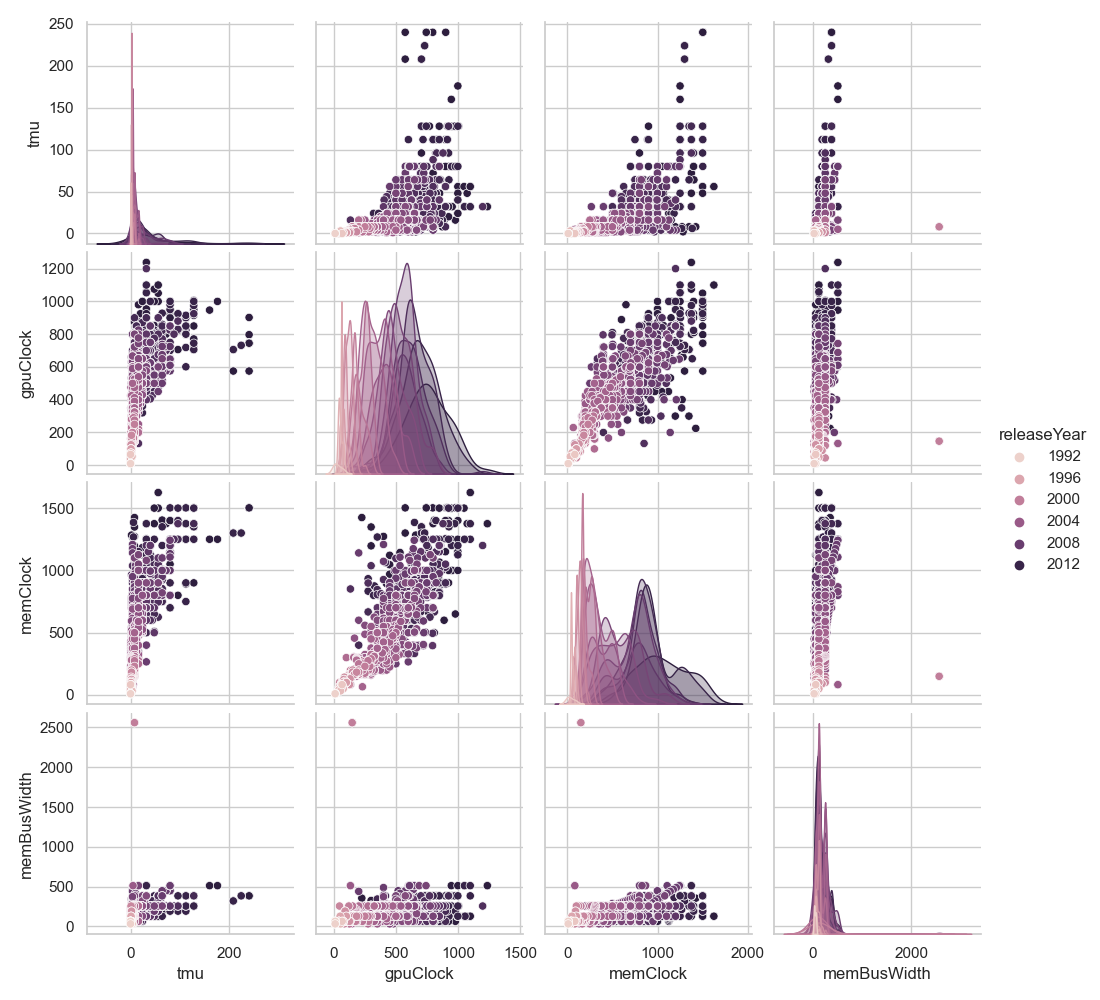
\includegraphics[width=0.7\textwidth]{Plots/DataPariPlot.png}
        \caption{Parallel plot of the data}
        \label{appdx:parallelPlotOfTheData}
    \end{figure}

    \begin{figure}
        \centering
        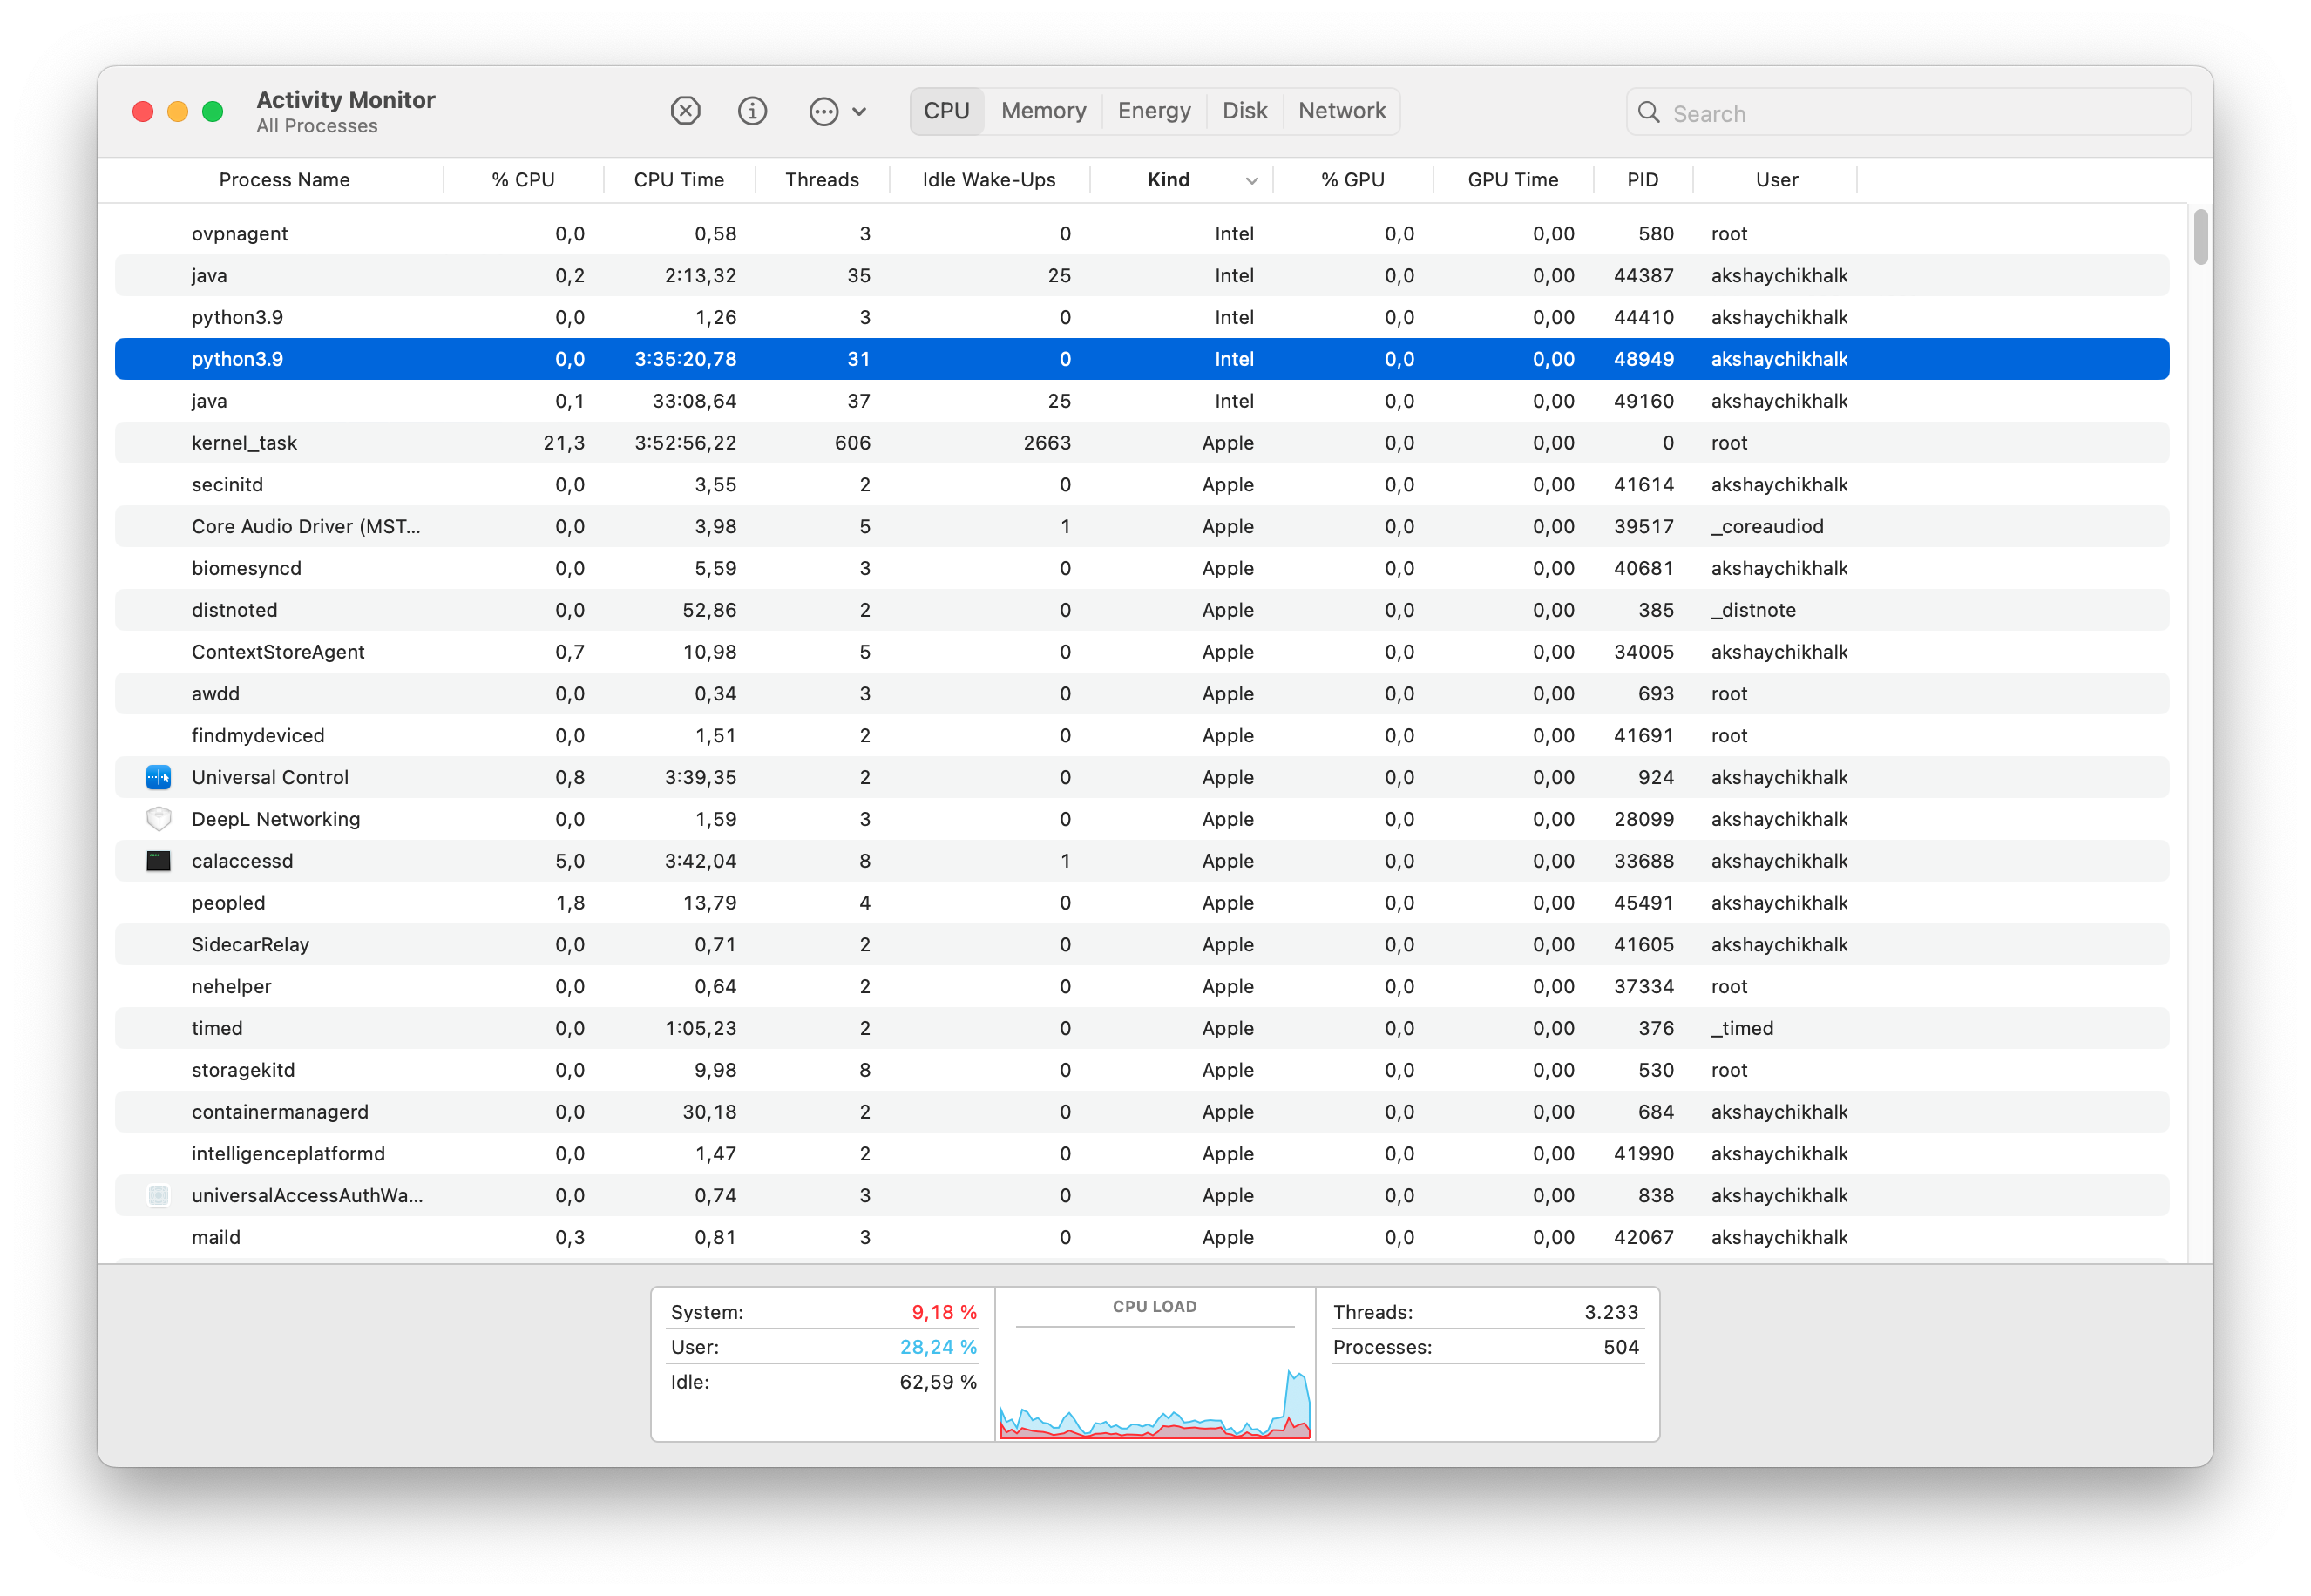
\includegraphics[width=0.7\textwidth]{ExucutionDetails.png}
        \caption{Execution details}
        \label{appdx:executionDetails}
    \end{figure}

\newpage
\bibliographystyle{IEEEtran}
\bibliography{ref}
\end{document}